\FloatBarrier
\chapter{Implementation}
\label{sec:implementation}

\section{Frontend}
\subsection{Architecture}
The frontend was implemented as a native web application using JavaScript, HTML, and CSS. Since the main modelling workflow is performed in the workspace page, only the workspace architecture is described here. The workspace follows a layered structure: UI modules handle rendering and user interaction, service modules coordinate the workflow logic, and store modules keep the client-side state synchronized across the document viewer, model editor, and project graph.

The workspace initialization logic validates the current project, loads the required UI modules, and triggers the initial data loading. At runtime, the workspace service loads document, model, and subprocess metadata, initializes the stores, and selects an initial document if available. Later actions, such as opening a version, generating a model, or navigating to a subprocess, are handled through the same orchestration flow.

\subsection{State Management}

The workspace presents four concurrently visible panes — the document list, document viewer, model editor, and project graph — each of which must react to changes triggered in the others. To keep these panes synchronized without coupling them directly, the frontend adopts a lightweight publish-subscribe mechanism: each pane subscribes to the stores it depends on and is notified whenever relevant state changes.

The mechanism is built around a small store hierarchy. The base \texttt{Store} class, shown in Figure~\ref{fig:imp_frontend_pubsub_store}, holds local state in a plain object and maintains a subscriber set. Specialized stores extend this foundation to cover different concerns: \texttt{EntitiesStore} manages keyed entity collections and exposes add, update, and remove operations; \texttt{VersionedEntityStore} further extends it with version-aware lookups; and separate stores for workspace coordination, document-viewer state, model-editor state, and the project graph each encapsulate their own domain fields and mutations.

\begin{figure}[H]
  \centering
  \caption{Base \texttt{Store} class implementing the publish-subscribe mechanism}
  \label{fig:imp_frontend_pubsub_store}
  \begin{lstlisting}[language=JavaScript]
export class Store {
  constructor(initialState = {}) {
    this.state = { ...initialState };
    this.subscribers = new Set();
  }

  subscribe(fn) {
    this.subscribers.add(fn);
    return () => this.subscribers.delete(fn);
  }

  notify(patch) {
    this.subscribers.forEach((fn) => fn(patch));
  }
}
  \end{lstlisting}
\end{figure}

UI modules interact with stores by calling \texttt{subscribe()} during initialization and holding the returned unsubscribe function for cleanup. Each notification delivers a patch object carrying a \texttt{key} and an \texttt{operation} field, so subscribers can react selectively — for example, the model-editor panel handles model-editor store patches while ignoring document-viewer updates. This targeted notification pattern supports synchronized updates across the workspace panes without requiring a larger frontend framework.

\subsection{Document Processing}
Document upload is partly handled on the frontend so that heterogeneous source formats can be normalized before entering the main interaction flow. The implementation accepts PDF, DOC, DOCX, and plain-text input. Word documents are converted to HTML using Mammoth.js\footnote{\url{https://github.com/mwilliamson/mammoth.js}, accessed 2026-04-15}, a client-side library that maps DOCX content to semantic HTML elements. PDF files are processed using PDF.js\footnote{\url{https://mozilla.github.io/pdf.js/}, accessed 2026-04-15}, Mozilla's open-source PDF rendering library, which provides access to the raw text content and its positional metadata.

For PDFs, the frontend uses PDF.js to extract per-page text items, then groups them into lines based on their vertical positions, classifies them as headings, list items, or paragraphs using font size and formatting heuristics, and assembles the result as semantic HTML. This normalization step is necessary because later operations — selection serialization, overlay rendering, and re-anchoring — depend on stable DOM text ranges rather than on raw file content.

\subsection{Text Selection Rendering}
One of the central frontend mechanisms is the transformation of browser text selections into persistent, version-aware linkable objects. A user selection is serialized into a text-position selector together with a text-quote selector, following the anchoring idea of the W3C Web Annotation Model \cite{w3c_annotation_model}. The text-position selector identifies the range in the current text stream, while the text quote preserves the selected wording for later validation or re-anchoring. Figure~\ref{fig:imp_frontend_selection_serialization} shows the core implementation used to convert a browser range into a persistent selector object.

\begin{figure}[H]
  \centering
  \caption{Core implementation of selection serialization}
  \label{fig:imp_frontend_selection_serialization}
  \begin{lstlisting}[language=JavaScript]
export function serializeRange(range) {
  const root = getRoot();
  const textPosition = textPos.fromRange(root, range);
  const textQuoteSelector = textQuote.fromTextPosition(root, textPosition);

  return {
    textPosition,
    textQuote: textQuoteSelector,
  };
}
  \end{lstlisting}
\end{figure}

When a stored selection is displayed again, the frontend resolves the serialized selector back into a DOM range. This allows existing links and older model versions to be visualized in the document viewer.

\subsubsection{Virtual Overlay Strategy}
Selection rendering is implemented as a virtual overlay rather than by wrapping the original text nodes. The selection module collects client rectangles, filters and de-duplicates them, removes oversized container rectangles, and reconstructs more accurate line-level rectangles when necessary. The resulting geometry is then rendered as overlay elements above the document content.
This avoids mutating the source DOM and keeps selection rendering stable across re-renders, updates, and version switches.

\subsubsection{Link Update Detection}
The frontend also distinguishes between semantic changes in a linked selection and purely visual updates. Link drafts are classified into three states: no change, color-only change, and text-changed. This distinction is important during document-version updates, where a visual modification should not invalidate the semantic relation between a passage and a model.

\subsection{Modeling}
The modeling flow coordinates the document viewer, the model service, and the model editor state. Selected text is aggregated, optionally combined with an additional prompt, and sent to the LLM-backed generation endpoint. The returned XML model data is then loaded into the model editor store and rendered in the editing pane.

The frontend also keeps the relation to the originating document version so that model editing remains synchronized with the document context. This logic supports new models, regenerations, refinements, and historical versions.

\subsection{Model Rendering Customization}
Instead of implementing a process-model editor from scratch, the frontend reuses the CPEE layout and rendering infrastructure and extends it where necessary. The main customization is the workflow adaptor layer, which dispatches additional events for call and subprocess nodes.

These events connect the generic renderer to workspace-specific behavior such as subprocess navigation and contextual interaction. Together, the layered frontend organization, pub-sub stores, document normalization, overlay rendering, and renderer customization support the end-to-end modelling workflow.

\section{Backend}
\subsection{Architecture}
The backend is implemented using a layered architecture. In this system, the layered structure is realized through route, service, and repository layers, each with a clearly separated responsibility. Route modules expose REST endpoints, service modules implement the application logic, and repository modules encapsulate data-access operations. Fastify.js was chosen as the backend framework because it is lightweight and provides native support for schema-based validation of requests and responses. 

The schema layer is important because the system exchanges structured selection data between frontend and backend. As shown in Figure~\ref{fig:imp_backend_schema_example}, selectors are validated before entering the service logic. The same approach is used across document, model, and link endpoints.

\begin{figure}[H]
  \centering
  \caption{Example JSON schema used in the backend for text quotes}
  \label{fig:imp_backend_schema_example}
  \begin{lstlisting}[language=JavaScript]
const textQuoteSchema = {
  type: "object",
  required: ["exact"],
  additionalProperties: false,
  properties: {
    exact: { type: "string" },
    prefix: { type: "string" },
    suffix: { type: "string" },
  },
};
  \end{lstlisting}
\end{figure}

The backend combines relational persistence with file-based storage. Metadata such as projects, documents, models, versions, and links are stored in SQLite, while large document contents and model XML payloads are stored as files in the persistence directory. This hybrid design keeps metadata queryable without placing large HTML and XML payloads directly in the database.

The service layer implements the application-specific workflows used by the frontend. For example, when a new document version is created, the backend stores the content, updates the latest-version pointer, and copies the latest link information. When a new model or model version is created, the backend persists the XML payload, updates version references, stores the related link, and records monitoring information. The backend also handles cross-cutting concerns such as soft deletion, logging, and aggregated workspace endpoints. 

\section{Database Schema}

Figure~\ref{fig:imp_data_model} illustrates the current data model of the system. Firstly, Project, Document, Model and DocumentModelLink are the minimal tables needed to support the proposed system. It is also how the system was implemented when it first adopted the database. The Document and Model tables were used to store metadata like name, words count of a document. Theoretically, the DocumentModelLink table can be stored as an attribute within the ModelVersion, since the system is currently designed to allow one model to be derived from only one document. But it is a decision made very early to store it in a separate table to easily support a potentially many-to-many (M2M) relationship in the future.

The ModelVersion table is added when the model versioning feature is about to be implemented. The DocumentVersion table is added at the same time to prepare for supporting the document update feature, as both tables follow a similar logic at the DB operation level. 

The SubprocessLink table is an additional table used to support the project graph. As this relationship information has been embedded in model data, the model visualization itself does not need this data. However, for the project graph, the relationship is hard to be parsed from the model data; therefore, such a table is implemented to easily retrieve the process-subprocess relationship.

The Selection and SelectionHistory tables are then added when designing the Document Update feature. Before the selection data (e.g., color, position) for a DocumentModelLink is stored as an attribute in the format of a stringified JSON object. To better support auto-reanchoring for document update, Selection and SelectionHistory are implemented as separate tables. The separate Selection table can make selection data easier to retrieve for reanchor operations. Besides, a Selection History is designed to make it easier to track the quality of reanchor. 

Finally, the GenerationAttempt and VersionEvent tables are the two tables needed to monitor the system behavior. The GenerationAttempt table is used to monitor the accept/decline decision for the LLM-generated output. The VersionEvent is mainly to store the manual edit behavior or a system auto-update behavior, e.g., selection reanchor for document update. 

\begin{figure}[htb!]
    \centering
    \caption{Data model}
    \floatfoot{Physical data model of the system with attributes omitted}
    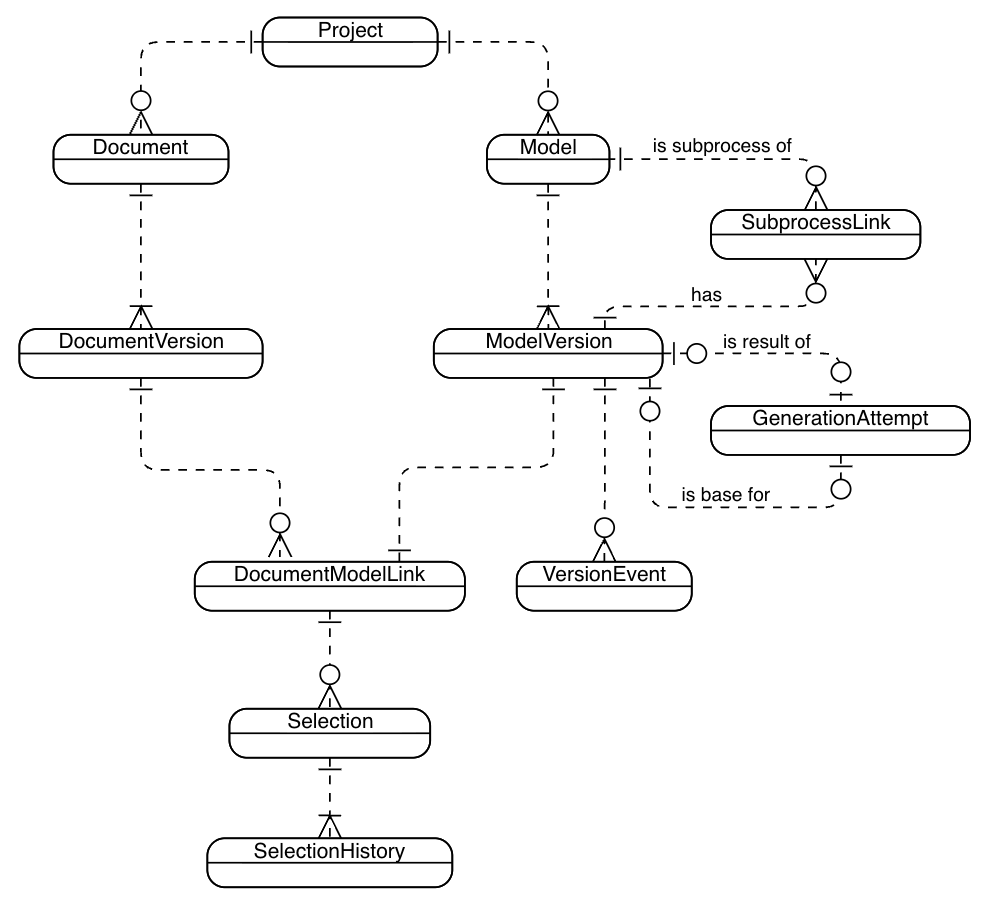
\includegraphics[width=1\textwidth]{images/imp_data_model.png}
    \label{fig:imp_data_model}
\end{figure}
